\newpage % Rozdziały zaczynamy od nowej strony.
\section{Analiza skuteczności algorytmów}

\subsection{Metody testowania}
\indent\ Testy zostały przeprowadzone za pomocą testów jednostkowych, w których wszystkie algorytmy zostały zestawione przeciwko sobie. Statki były rozstawiane losowo dla obu stron, z wyjątkiem testów w których analizowany był wpływ rozstawienia statków na skuteczność. Wszystkie testy jednostkowe dziedziczą po klasie bazowej \emph{AlgorithmTestBase}, która była potrzebna do inicjalizacji lub zmockowania wszelkich potrzebnych serwisów. Na listingu 12 widoczny jest przykładowy test jednostkowy. Testowane były oba warianty zasady stykania się statków. Stała \emph{numberOfIterations} wynosiła 1000, więc dla każdego zestawienia algorytmów i zasad otrzymano 1000 wyników. Ogólnie podczas testów zebrano około 240 000 rekordów w kontenerze \emph{TestGameSessions}.

\begin{addmargin}[10mm]{0mm}
\begin{lstlisting}[
    language={[Sharp]C},
    numbers=left,
    firstnumber=11,
    caption={Przykładowy test jednostkowy},
    aboveskip=0pt
]
[Fact]
public void VsRandomShipsCantTouch()
{
    _httpContextAccessor.SetupTestHttpContext();

    var initialGameState = new GameState
    {
        PlayerAiType = AiType.LocationHeuristic,
        OpponentAiType = AiType.Random,
        ShipsCanTouch = false,
    };

    var playerWins = TestHelper.RunSimulation(
        initialGameState,
        _gameStateService,
        _generateMoveService,
        _shipLocationService,
        numberOfIterations);

    Assert.True(true);
}
\end{lstlisting}
\end{addmargin}


\subsection{Badanie skuteczności algorytmów przeciwko sobie}
W tabelach widocznych w poniższych rozdziałach stosowane będą skrócone nazwy algorytmów, tak aby bez problemu mieściły się w komórkach tabel. Poniżej znajduje się objaśnienie skrótów.
\begin{itemize}
    \item \textbf{Max. zysk} - Algorytm oparty na heurystyce maksymalizacji zysku ze strzału.
    \item \textbf{Analiza trafień} - Algorytm oparty na heurystyce najbardziej prawdopodobnej lokalizacji na podstawie trafień.
    \item \textbf{Max. zysk rozszerzony} - Algorytm oparty na heurystyce maksymalizacji zysku priorytetyzującej dłuższe statki.
    \item \textbf{Max. zysk + analiza trafień} - Algorytm oparty na heurystykach maksymalizacji zysku oraz najbardziej prawdopodobnej lokalizacji na podstawie trafień.
    \item \textbf{Max. zysk rozszerzony + analiza trafień} - Algorytm oparty na heurystykach maksymalizacji zysku oraz najbardziej prawdopodobnej lokalizacji na podstawie trafień priorytetyzującej dłuższe statki. 
\end{itemize}

W tabelach przedstawiających skuteczność poszczególnych algorytmów posłużono się kolorami, w celu podkreślenia otrzymanych wartości:
\begin{itemize}
    \item Kolor zielony - wynik zdecydowanie lepszy, skuteczność powyżej 55\%
    \item Kolor żółty - wynik porównywalny, skuteczność pomiędzy 45\%-55\%
    \item Kolor czerwony - wynik zdecydowanie gorszy, skuteczność poniżej 45\%
\end{itemize}

\subsubsection{Algorytm losowy}

Algorytm losowy, zgodnie z przewidywaniami wypadł najgorzej w zestawieniu z innymi algorytmami. Z tabeli 7.1 wynika, że najwyższy procent zwycięstw jaki osiągnął to 13,1\% przeciwko algorytmowi losowemu rozszerzonemu. Wśród wyników można zaobserwować prawidłowość, że skuteczność delikatnie wzrasta w przypadku testów, gdzie statki mogą się stykać. Zgodnie z tym, co opisano pod koniec rozdziału 2.2, dodatkowe ograniczenie tego, jak mogą być rozstawione statki, ułatwia heurystykom analizę planszy przeciwnika. Gdy tego ograniczenia nie ma, gra staje się trochę bardziej losowa - chociaż nadal algorytmy oparte na heurystykach są znacznie skuteczniejsze od algorytmu losowego.

\begin{table}[!h]
    \centering
    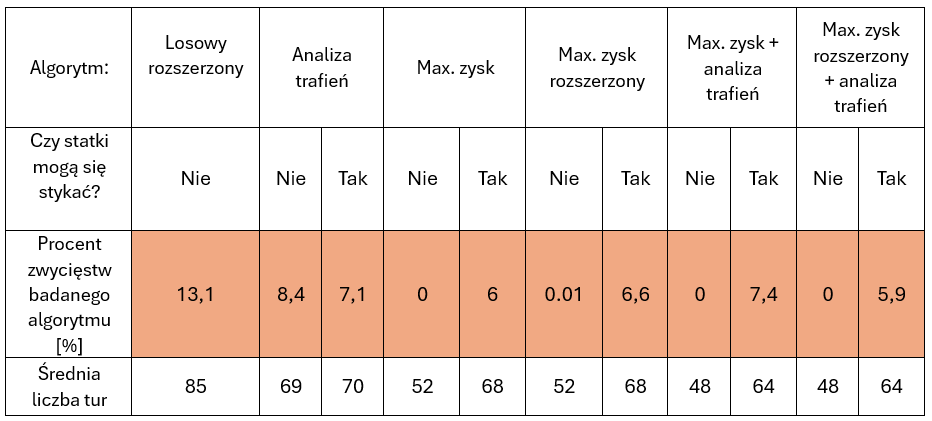
\includegraphics[width=1\linewidth]{img/table-random.png}
    \caption{Wyniki testów dla algorytmu losowego}
\end{table}

\subsubsection{Algorytm losowy z pominięciem pól sąsiadujących z zatopionymi statkami}

Algorytm losowy z pominięciem pól był testowany jedynie w przypadku gdy statki nie mogą się ze sobą stykać. W przeciwnym wypadku, gdyby oponent ustawił statki obok siebie, badany algorytm nie byłby w stanie odnieść zwycięstwa. W wynikach testów widocznych w tabeli 7.2 widać, że algorytm rozszerzony jest dużo skuteczniejszy od swojej podstawowej wersji. Można też zauważyć zdecydowany wzrost skuteczności przeciwko algorytmowi opartemu na heurystyce najbardziej prawdopodobnej lokalizacji na podstawie trafień. W pozostałych przypadkach również można zaobserwować wzrost skuteczności, ale jest on bardzo niewielki.

\begin{table}[!h]
    \centering
    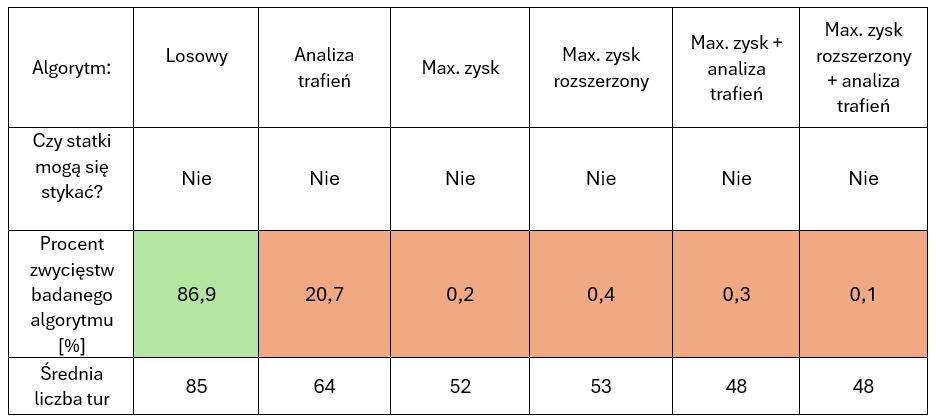
\includegraphics[width=1\linewidth]{img/table-random-plus.png}
    \caption{Wyniki testów dla algorytmu losowego rozszerzonego}
\end{table}

\subsubsection{Algorytm oparty na heurystyce najbardziej prawdopodobnej lokalizacji na podstawie trafień}

Z tabeli 7.3 wynika, że w przypadku tego algorytmu widoczna jest wyraźnie jego przewaga nad algorytmami losowymi. Jest on jednak zdecydowanie najsłabszym z algorytmów heurystyczych. Umiejętność 'dobijania' trafionych statków wyróżnia go na tle algorytmów losowych, ale nadal w dużej mierze opiera się na losowości - jeśli na planszy przeciwnika nie ma żadnego trafienia, algorytm oddaje strzały w losowe komórki.

Podobnie jak w 7.2.1, widać znaczącą różnicę w zależności od wyboru zasad - skuteczność tego algorytmu wzrasta gdy statki mogą się ze sobą stykać.

\begin{table}[!h]
    \centering
    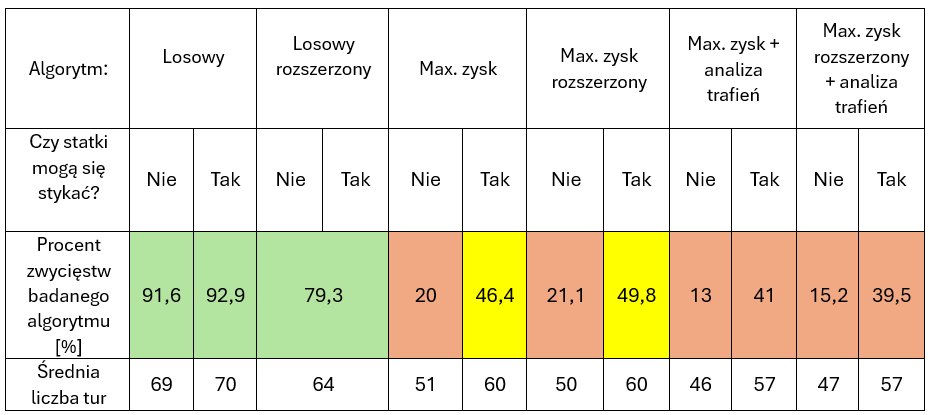
\includegraphics[width=1\linewidth]{img/table-hit-heuristic.png}
    \caption{Wyniki testów dla algorytmu opartego na heurystyce najbardziej prawdopodobnej lokalizacji na podstawie trafień}
\end{table}

\subsubsection{Algorytm oparty na heurystyce maksymalizacji zysku ze strzału}

W przypadku tego algorytmu widać wzrost skuteczności o około 10\% względem algorytmów losowych. Algorytm ten jest też zdecydowanie skuteczniejszy od algorytmu opartego na heurystyce najbardziej prawdopodobnej lokalizacji na podstawie trafień, aczkolwiek gdy statki mogą się ze sobą stykać, to ich skuteczność jest porównywalna.

\begin{table}[!h]
    \centering
    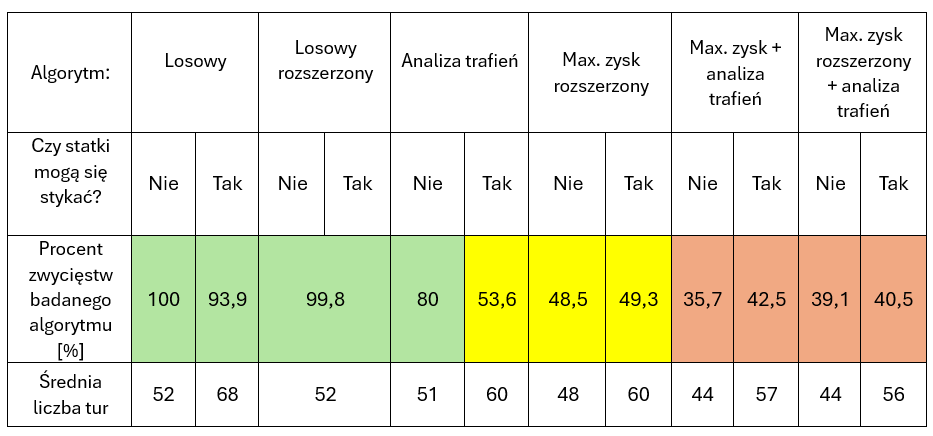
\includegraphics[width=1\linewidth]{img/table-location-heuristic.png}
    \caption{Wyniki testów dla algorytmu opartego na heurystyce maksymalizacji zysku ze strzału}
\end{table}


\subsubsection{Algorytm oparty na heurystyce maksymalizacji zysku priorytetyzującej dłuższe statki}

Wyniki zaprezentowane w tabeli 7.5 są bardzo zbliżone do wartości z punktu 7.2.4. Można zaobserwować, że w bezpośrednim starciu, badany algorytm jest nieznacznie skuteczniejszy od swojego podstawowego wariantu. Jednak we wszystkich pozostałych przypadkach, poza jednym, widoczny jest nieznaczny spadek skuteczności, w najgorszym przypadku 3,5\%.

\begin{table}[!h]
    \centering
    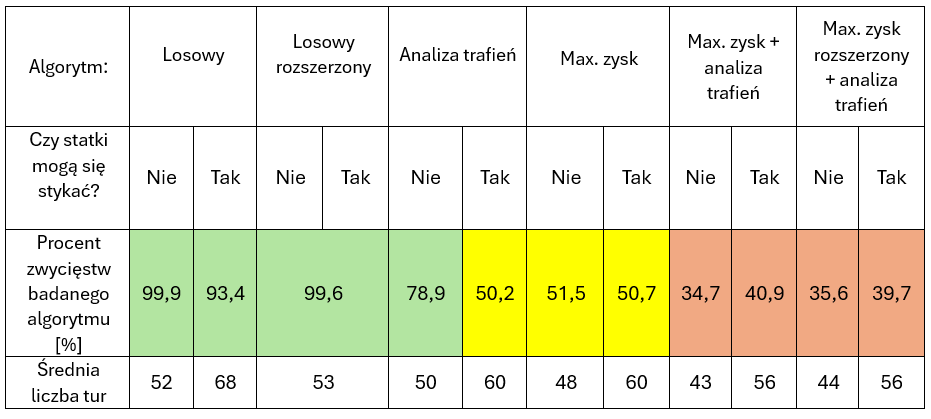
\includegraphics[width=1\linewidth]{img/table-location-heuristic-extended.png}
    \caption{Wyniki testów dla algorytmu opartego na heurystyce maksymalizacji zysku priorytetyzującej dłuższe statki}
\end{table}

\subsubsection{Algorytm oparty na heurystykach maksymalizacji zysku oraz najbardziej prawdopodobnej lokalizacji na podstawie trafień}

Jak wynika z danych w tabeli 7.6, algorytm wygrywa w zestawieniu ze wszystkimi pozostałymi algorytmami, poza swoją rozszerzoną wersją. Największy wzrost skuteczności widać przeciwko algorytmom \emph{Analiza trafień} oraz \emph{Max.zysk}. Wynika to z faktu, że badany algorytm jest usprawnieniem \emph{Max.zysk} poprzez umożliwienie algorytmowi 'dobijania' trafionych statków.

\begin{table}[!h]
    \centering
    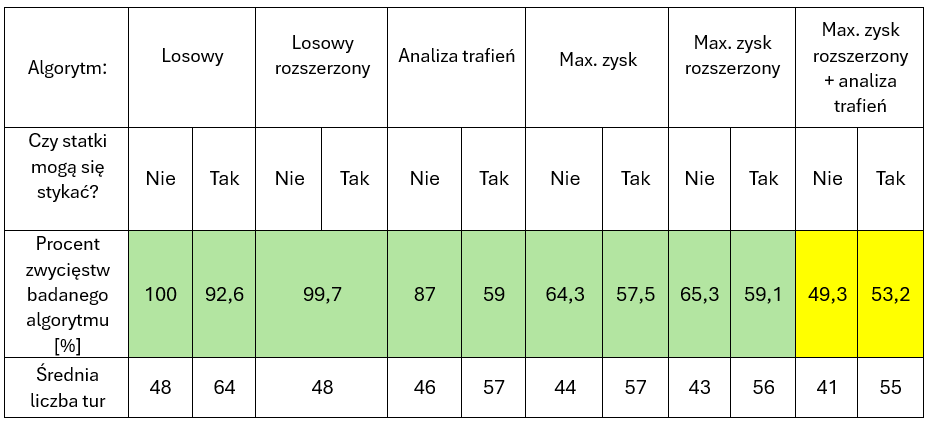
\includegraphics[width=1\linewidth]{img/table-location-hit-heuristic.png}
    \caption{Wyniki testów dla algorytmu opartego na heurystykach maksymalizacji zysku oraz najbardziej prawdopodobnej lokalizacji na podstawie trafień}
\end{table}

\subsubsection{Algorytm oparty na heurystykach maksymalizacji zysku oraz najbardziej prawdopodobnej lokalizacji na podstawie trafień priorytetyzującej dłuższe statki}

Podobnie jak w przypadku 7.2.5, wyniki wersji podstawowej i rozszerzonej algorytmu są bardzo zbliżone. W bezpośrednim starciu wersja rozszerzona jest nieznacznie skuteczniejsza, gdy statki nie mogą się ze sobą stykać. W przeciwnym wypadku, lepiej wypada wersja podstawowa algorytmu. W starciach z pozostałymi algorytmami wyniki są zbliżone.

\begin{table}[!h]
    \centering
    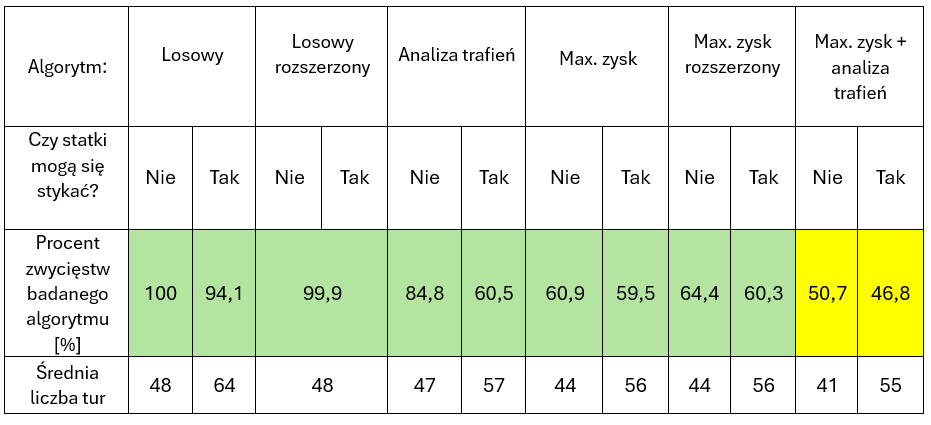
\includegraphics[width=1\linewidth]{img/table-location-extended-hit-heuristic.png}
    \caption{Wyniki testów dla algorytmu opartego na heurystykach maksymalizacji zysku oraz najbardziej prawdopodobnej lokalizacji na podstawie trafień priorytetyzującej dłuższe statki}
\end{table}

\subsection{Podsumowanie}

Aby wyłonić najskuteczniejszy algorytm, utworzono tabele 7.8 oraz 7.9. Przedstawiają one zestawienie pojedynków pomiędzy wszystkimi algorytmami. Tabela 7.8 przedstawia wyniki, gdy statki nie mogą się ze sobą stykać, a tabela 7.9. przeciwny przypadek. W każdej kolumnie na zielono zaznaczone zostały komórki zawierające najwyższą skuteczność. Oznacza to, że algorytm przypisany do danego wiersza, był najskuteczniejszy w starciu z algorytmem przypisanym do danej kolumny.

Analizując dane tabel 7.8 i 7.9, można zaobserwować, że:

\begin{itemize}
    \item Gdy statki nie mogą się ze sobą stykać, podstawowa wersja  \emph{Max. zysk + analiza trafień} jest najskuteczniejsza w prawie wszystkich przypadkach. 
    \item Gdy statki mogą się ze sobą stykać, rozszerzona wersja  \emph{Max. zysk + analiza trafień} jest najskuteczniejsza w prawie wszystkich przypadkach, poza bezpośrednim starciem ze swoją podstawową wersją.
\end{itemize}

Widać więc wyraźnie wpływ różnicy zasad na wyniki. Ciekawe jest to, że w obu przypadkach ogólnie najskuteczniejszy algorytm przegrywał w starciu ze swoim drugim wariantem.

Aby ostatecznie rozstrzygnąć, który algorytm jest bardziej skuteczny spróbowano również policzyć ich ogólną skuteczność. Dokonano tego poprzez obliczenie średniej ze skuteczności przeciwko poszczególnym algorytmom. Przekłada się to na następujące wyniki procentowe:

\begin{itemize}
    \item 70,94\% dla wersji podstawowej
    \item 70,51\% dla wersji rozszerzonej
\end{itemize}

Nieznacznie skuteczniejszy jest więc wersja podstawowa \emph{Max. zysk + analiza trafień}.
\begin{table}[!h]
    \centering
    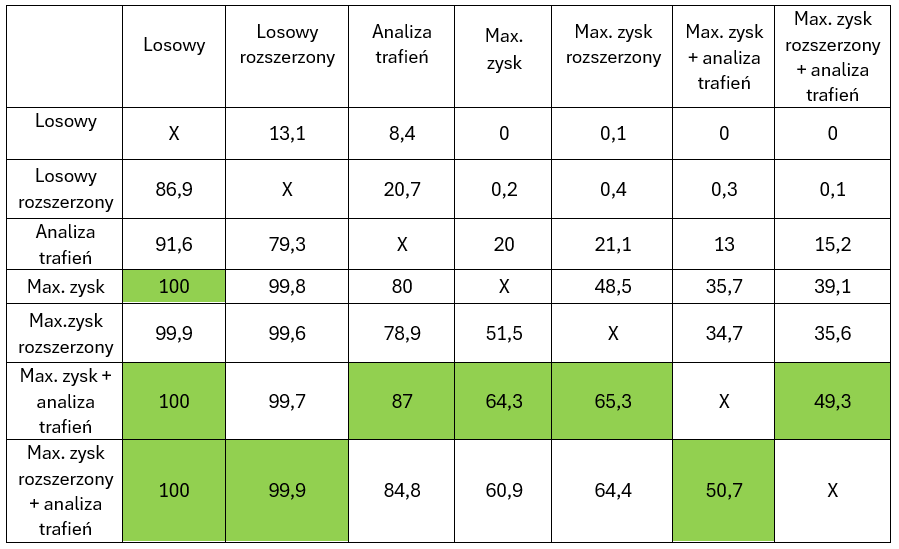
\includegraphics[width=1\linewidth]{img/summary-ships-cant-touch.PNG}
    \caption{Podsumowanie testów gdy statki nie mogą się ze sobą stykać}
\end{table}

\begin{table}[!h]
    \centering
    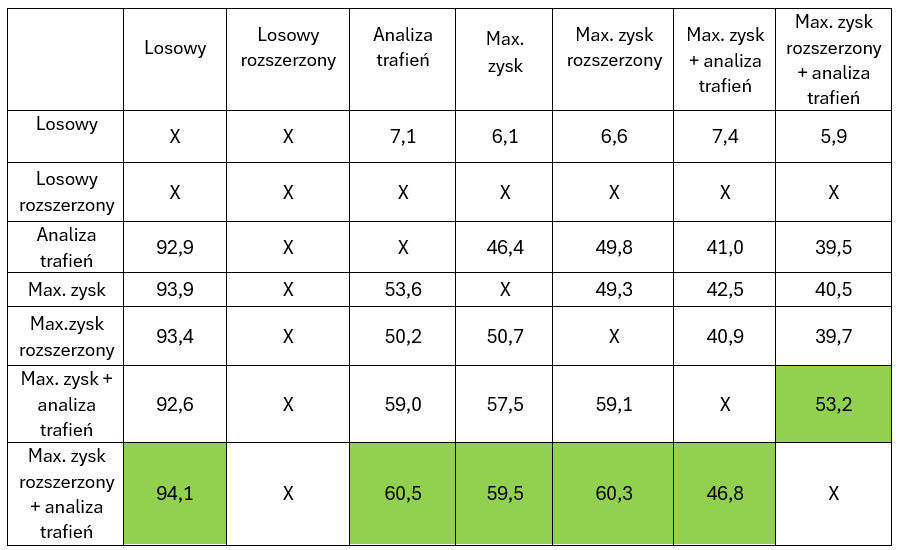
\includegraphics[width=1\linewidth]{img/summary-ships-can-touch.PNG}
    \caption{Podsumowanie testów gdy statki mogą się ze sobą stykać}
\end{table}

Analogicznie obliczono zagregowane skuteczności dla wszystkich algorytmów, co przedstawia tabela 7.10. Przy obliczeniach wykorzystano zapytanie widoczne na listingu 13.

\begin{table}[!h]
    \centering
    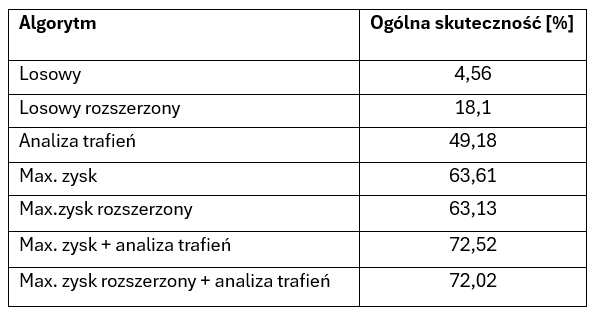
\includegraphics[width=0.7\linewidth]{img/aggregate.PNG}
    \caption{Zagregowane średnie skuteczności poszczególnych algorytmów}
\end{table}

\begin{addmargin}[10mm]{0mm}
\begin{lstlisting}[
    language=SQL,
    numbers=left,
    firstnumber=1,
    caption={Zapytanie do Azure Cosmos DB, w celu uzyskania zagregowanej skuteczności algorytmu},
    aboveskip=0pt
]
SELECT 
    AVG(
        IIF(c.playerMovesCount > c.opponentMovesCount,
        c.playerMovesCount,
        c.opponentMovesCount)
    ) AS avgMaxMoves
FROM c
WHERE (c.playerAiType = {ALG_1} AND c.opponentAiType = {ALG_2}
OR c.playerAiType = {ALG_2} AND c.opponentAiType = {ALG_1})
and c.shipsCanTouch = {WYBRANE_ZASADY}
\end{lstlisting}
\end{addmargin}

Na podstawie wyników stworzono wykres widoczny na rysunku 7.1. Algorytmy zostały posortowane od najmniej do najbardziej skutecznego.

\begin{figure}[!h]
    \label{fig:aggregate-chart}
    \centering 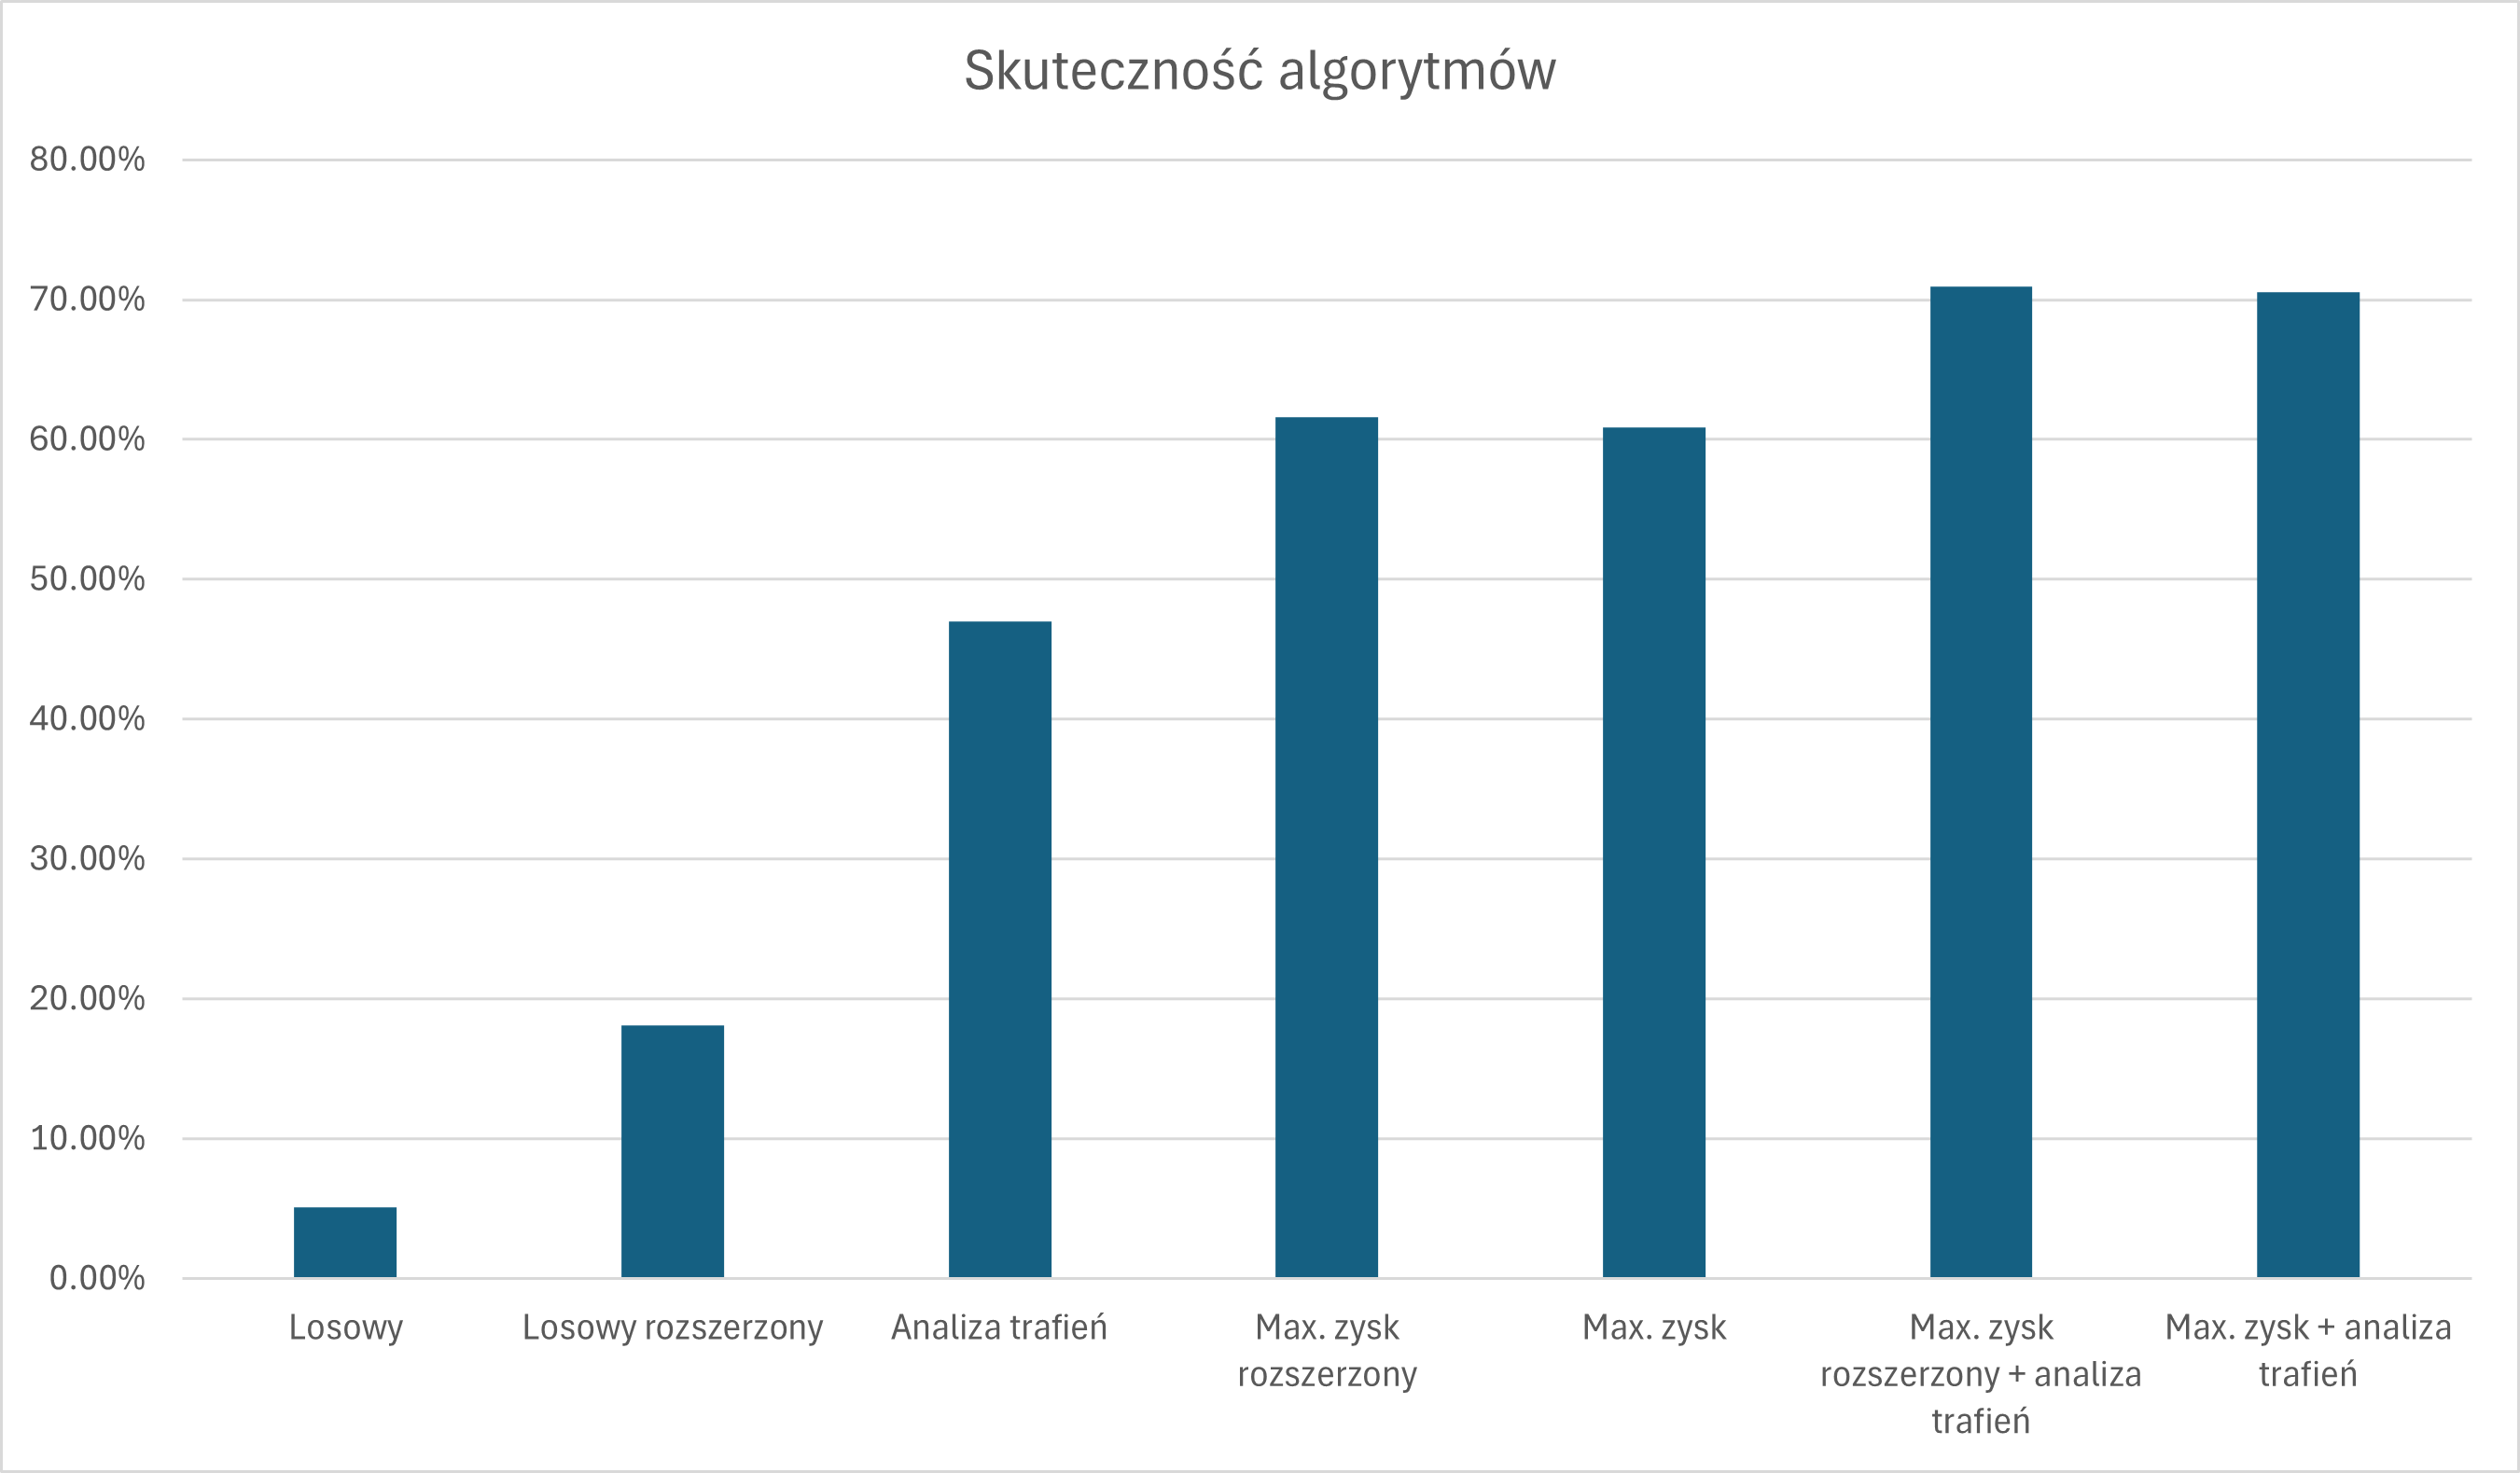
\includegraphics[width=0.9\linewidth]{img/aggregate-chart.png}
    \caption{Wykres zagregowanych średnich dla poszczególnych algorytmów.}
\end{figure}

Utworzono również wykres 7.2 obrazujący skuteczności różnych algorytmów w starciach z algorytmem losowym, aby lepiej zobrazować różnice w skuteczności, zależnie od tego czy statki mogą się ze sobą stykać, czy nie.

\begin{figure}[!h]
    \label{fig:round-avg}
    \centering 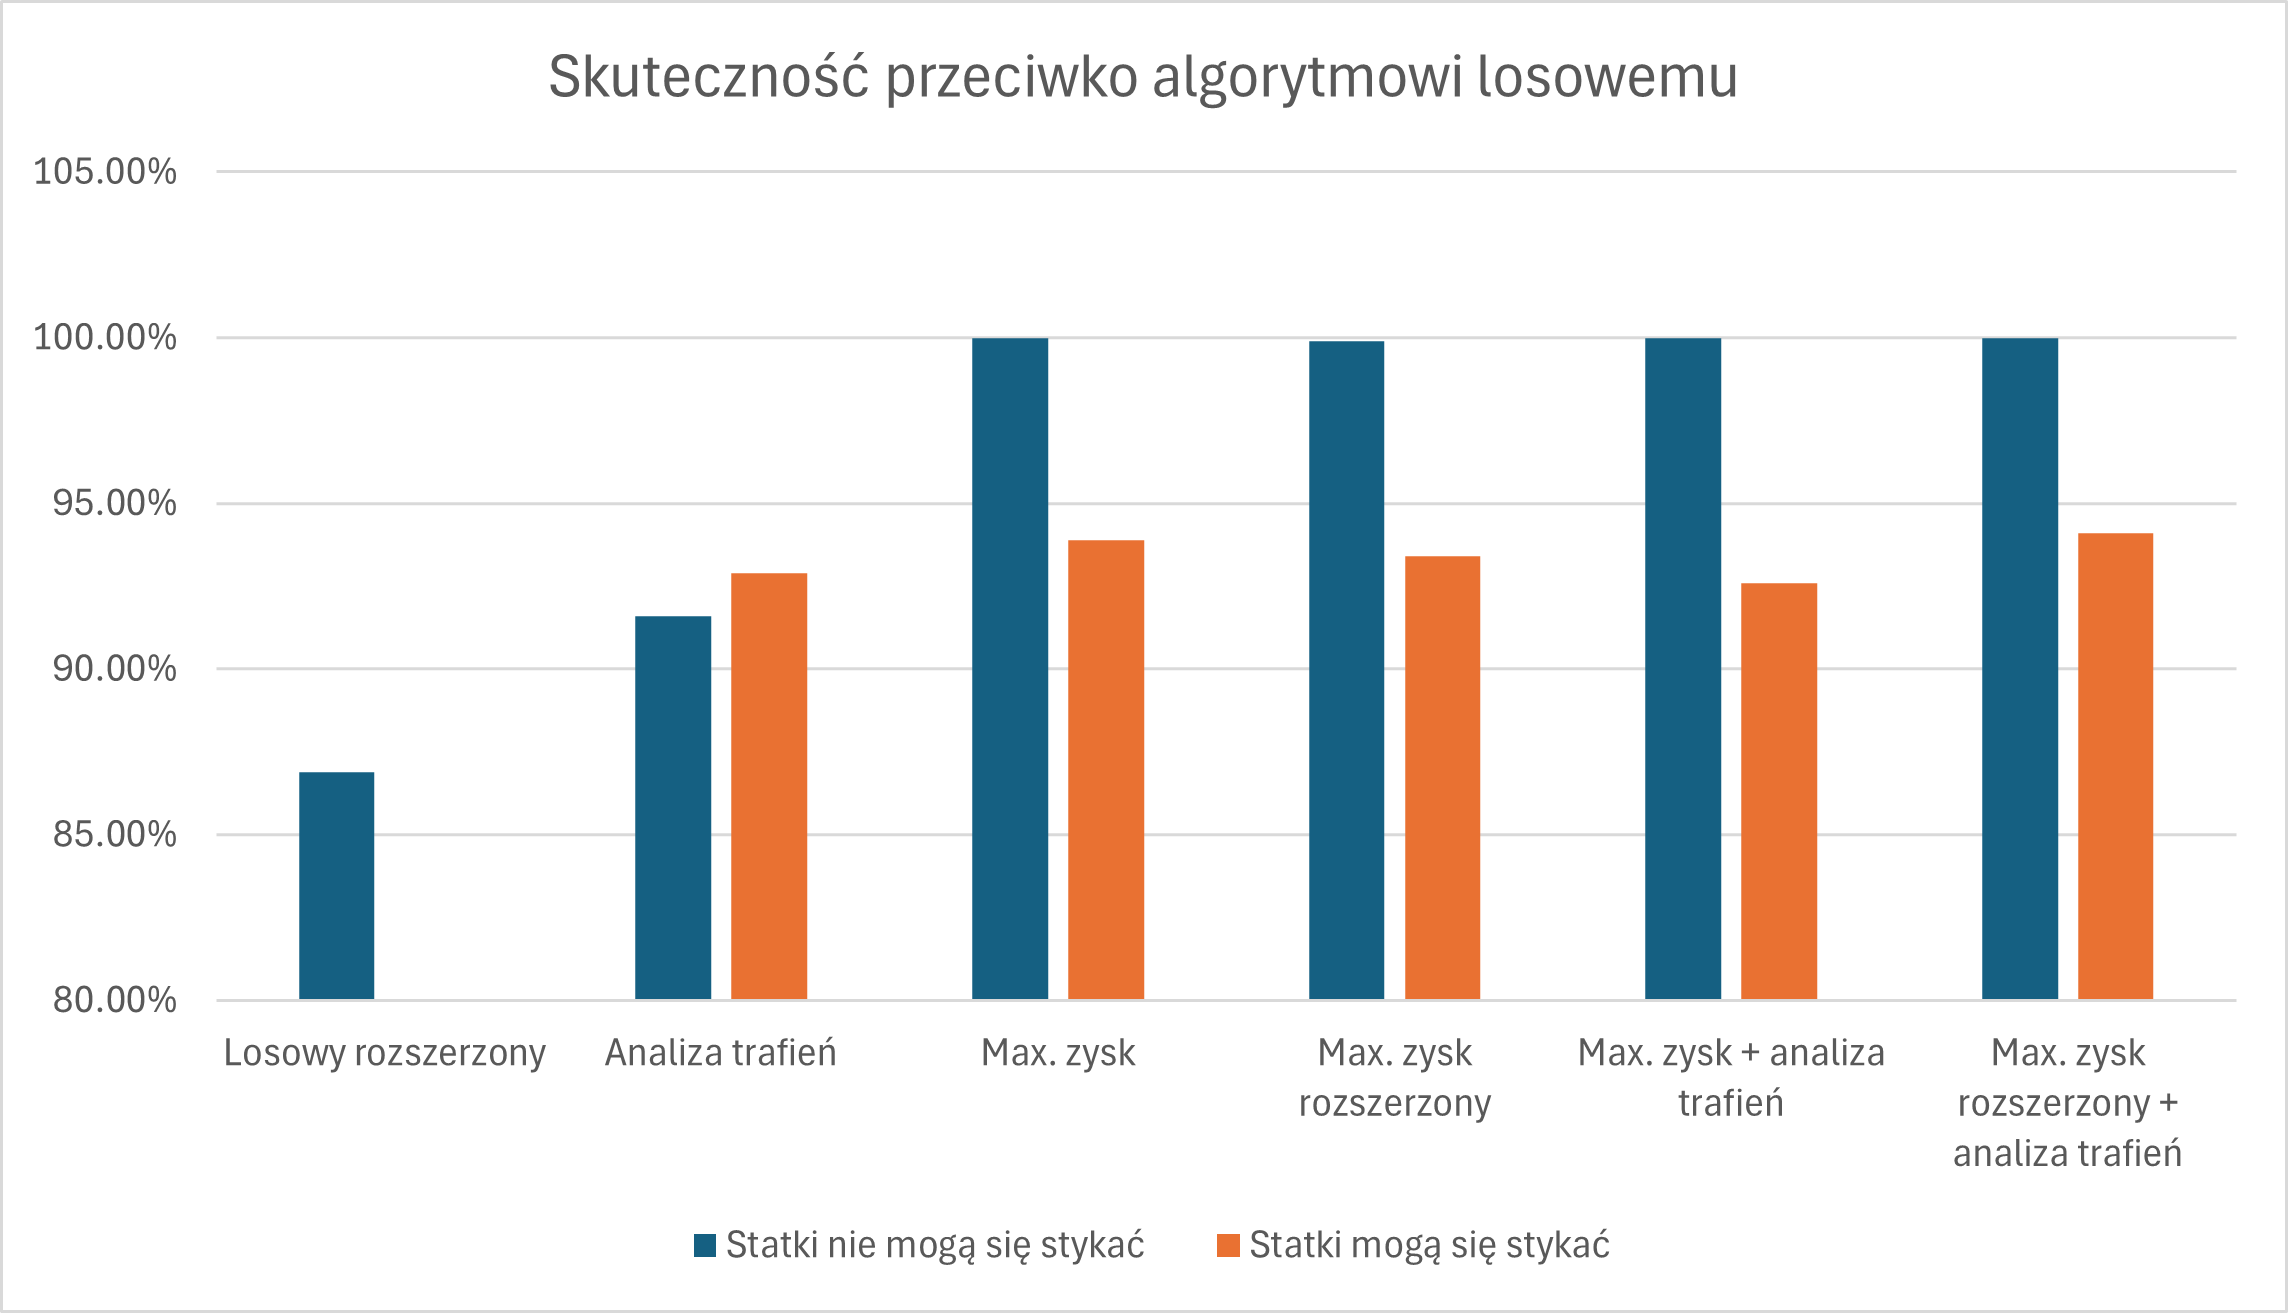
\includegraphics[width=0.9\linewidth]{img/chart-random-scores.png}
    \caption{Skuteczność algorytmów w starciach z algorytmem losowym.}
\end{figure}

Dla wszystkich zestawień algorytmów obliczono również średnią liczbę zagranych tur, zanim jedna ze stron odniosła zwycięstwo. Dane te widoczne są w tabelach 7.1-7.9 oraz na wykresie z rysunku 7.3, gdzie jako punkt odniesienia wykorzystano algorytm losowy.

\begin{figure}[!h]
    \label{fig:round-avg}
    \centering 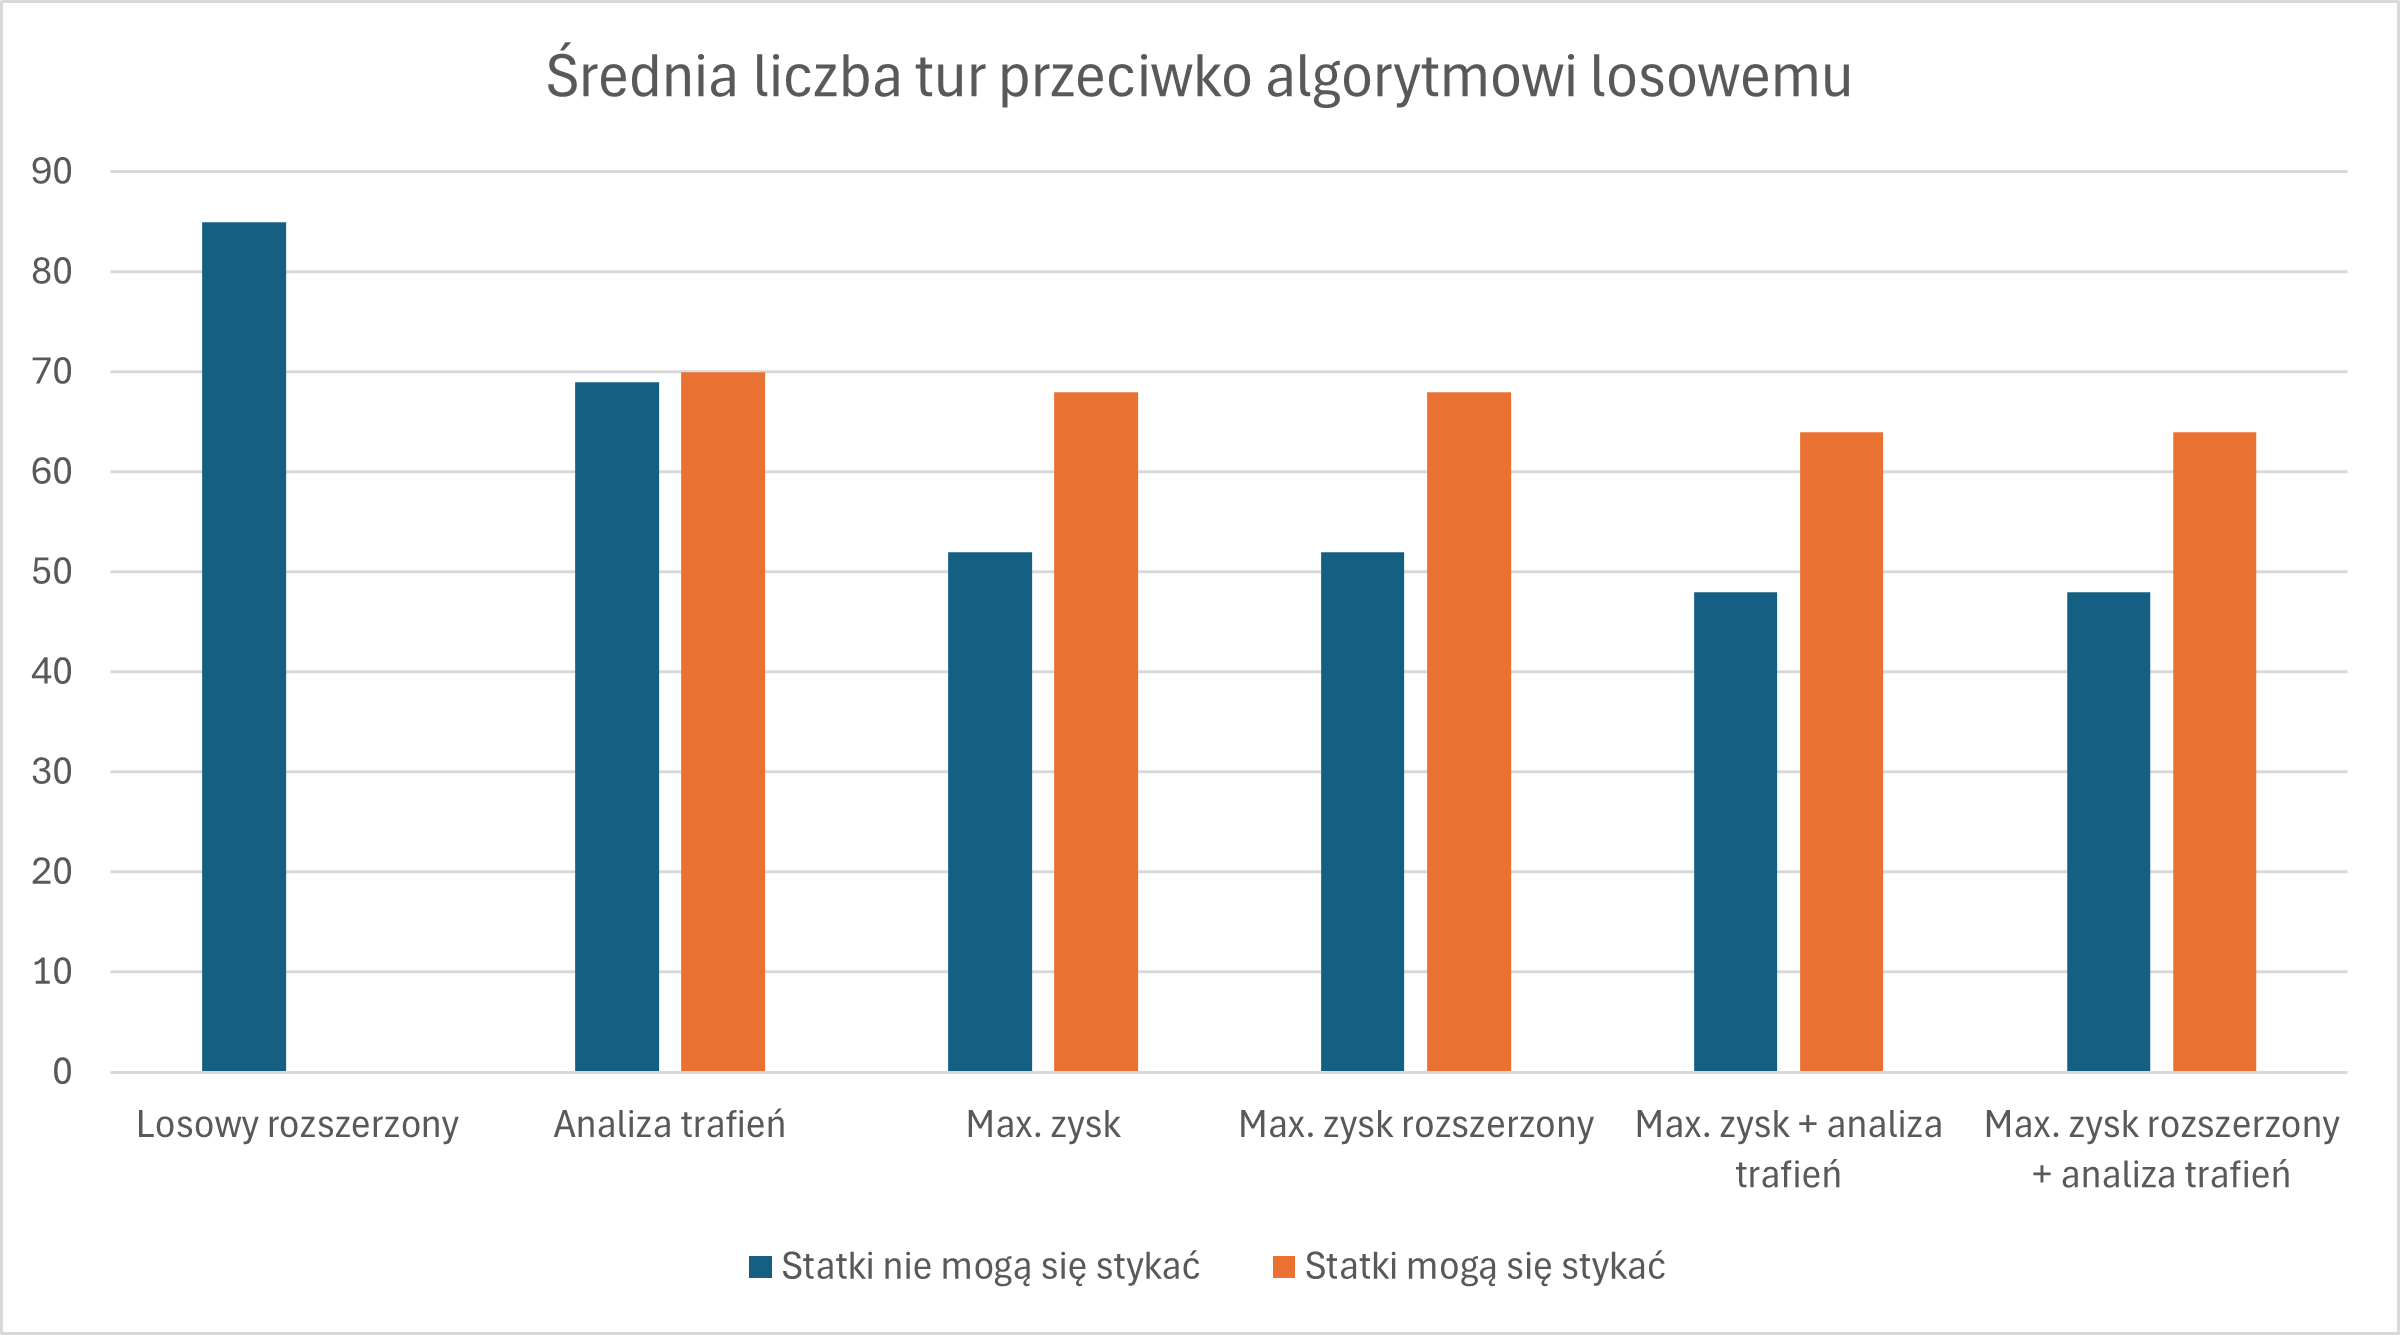
\includegraphics[width=0.9\linewidth]{img/round-count-avg.png}
    \caption{Średnia liczba tur w starciach z algorytmem losowym.}
\end{figure}

\subsection{Badanie wpływu liczby statków na skuteczność algorytmów}
Aby zbadać wpływ liczby statków na skuteczność algorytmów, powtórzone testy najbardziej skutecznego algorytmu \emph{Max. zysk + Analiza trafień}, w 3 różnych wariantach:
\begin{itemize}
    \item Obie strony mają do dyspozycji dodatkowe 2 jednomasztowce.
    \item Obie strony mają do dyspozycji dodatkowy pięciomasztowiec oraz czteromasztowiec.
    \item Obie strony mają do dyspozycji dodatkowe 2 trzymasztowce.
\end{itemize}

W tabelach w kolejnych podrozdziałach komórki tabel oznaczane są na czerwono, jeśli spadek skuteczności przekracza 5\%, na zielono jeśli wzrost jest większy od 5\% oraz na żółto jeśli zmiana skuteczności mieści się pomiędzy -5\% i 5\%.

\subsubsection{Dodatkowe najmniejsze statki}

W tabeli 7.11 widać wyraźny spadek skuteczności \emph{Max. zysk + Analiza trafień} w większości przypadków poza \emph{Analizą trafień}. Liczba tur wymaganych do zwycięstwa wzrasta, co było łatwe do przewidzenia, jako że obie strony mają teraz więcej statków do zestrzelenia.

\begin{table}[!h]
    \label{fig:vs-people}
    \centering 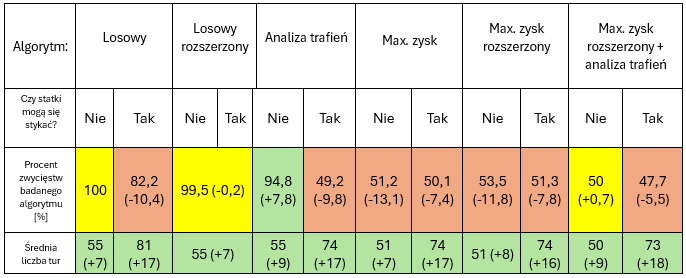
\includegraphics[width=0.9\linewidth]{img/shipCountSmallShips.png}
    \caption{Skuteczność \emph{Max. zysk + Analiza trafień} przy dodatkowych jednomasztowcach.}
\end{table}

\subsubsection{Dodatkowe średnie statki}

W tabeli 7.12 widzimy, że skuteczność algorytmu jest bardzo zbliżona do skuteczności przy 'normalnej' liczbie statków. Po raz kolejny widoczny jest wzrost skuteczności przeciwko \emph{Analizie trafień}.

\begin{table}[!h]
    \label{fig:vs-people}
    \centering 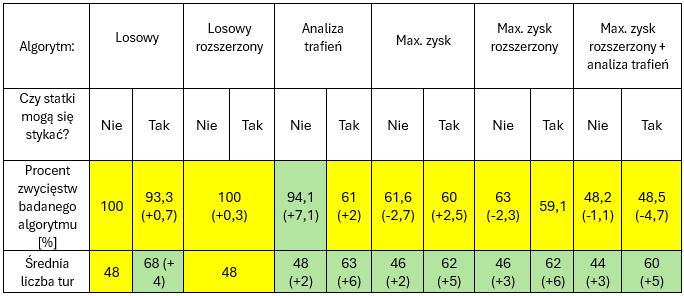
\includegraphics[width=0.9\linewidth]{img/shipCountMiddleShips.png}
    \caption{Skuteczność \emph{Max. zysk + Analiza trafień} przy dodatkowych trzymasztowcach.}
\end{table}

\subsubsection{Dodatkowe największe statki}

Podobnie do poprzedniego podpunktu, w tabeli 7.13 widać, że skuteczność \emph{Max. zysk i analiza trafień} jest zbliżona do  skuteczności przy 'normalnej' liczby statków. Znowu widać wzrost skuteczności przeciwko \emph{Analizie trafień}. Co ciekawe, w kilku przypadkach liczba tur jest mniejsza niż w przy 'normalnej' liczbie statków.

\begin{table}[!h]
    \label{fig:vs-people}
    \centering 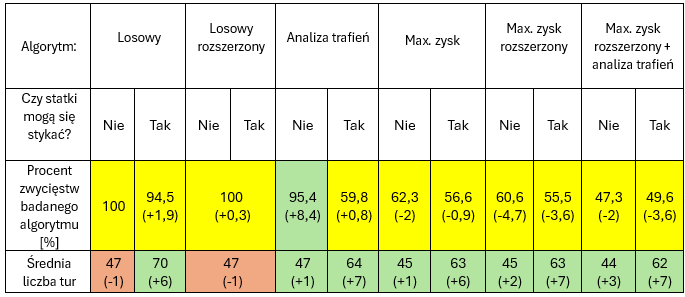
\includegraphics[width=0.9\linewidth]{img/shipCountBigShips.png}
    \caption{Skuteczność \emph{Max. zysk + Analiza trafień} przy dodatkowych cztero- i pięciomasztowcu.}
\end{table}

\subsection{Badanie wpływu rozstawienia statków na skuteczność algorytmów}
Postanowiono zbadać również wpływ rozstawienia statków na skuteczność algorytmów. W tym celu przeprowadzono analizę starć pomiędzy identycznymi algorytmami w 4 przypadkach:

\begin{itemize}
    \item Gdy statki są rozstawiane losowo przez obie strony.
    \item Gdy jedna ze stron częściej ustawia statki w narożnikach planszy.
    \item Gdy jedna ze stron częściej ustawia statki po lewej stronie planszy.
    \item Gdy jedna ze stron częściej ustawia statki w centrum planszy.
\end{itemize}

W tym celu zmodyfikowano kod odpowiadający za losowe rozstawianie statków, tak aby dla każdego statku istniało 80\% szans, że zostanie ustawiony w preferowanym obszarze planszy.

Korzystając ze skryptów \emph{GetShipLocations.py} oraz \emph{getData.py}, dostępnych w załączniku 3, wygenerowane zostały mapy cieplne widoczne na rysunku 7.4. Przedstawiają one to jak często dana komórka była częścią statku - im ciemniejszy kolor, tym częściej.

\begin{figure}[!h]
    \label{fig:bias-benchmark}
    \centering 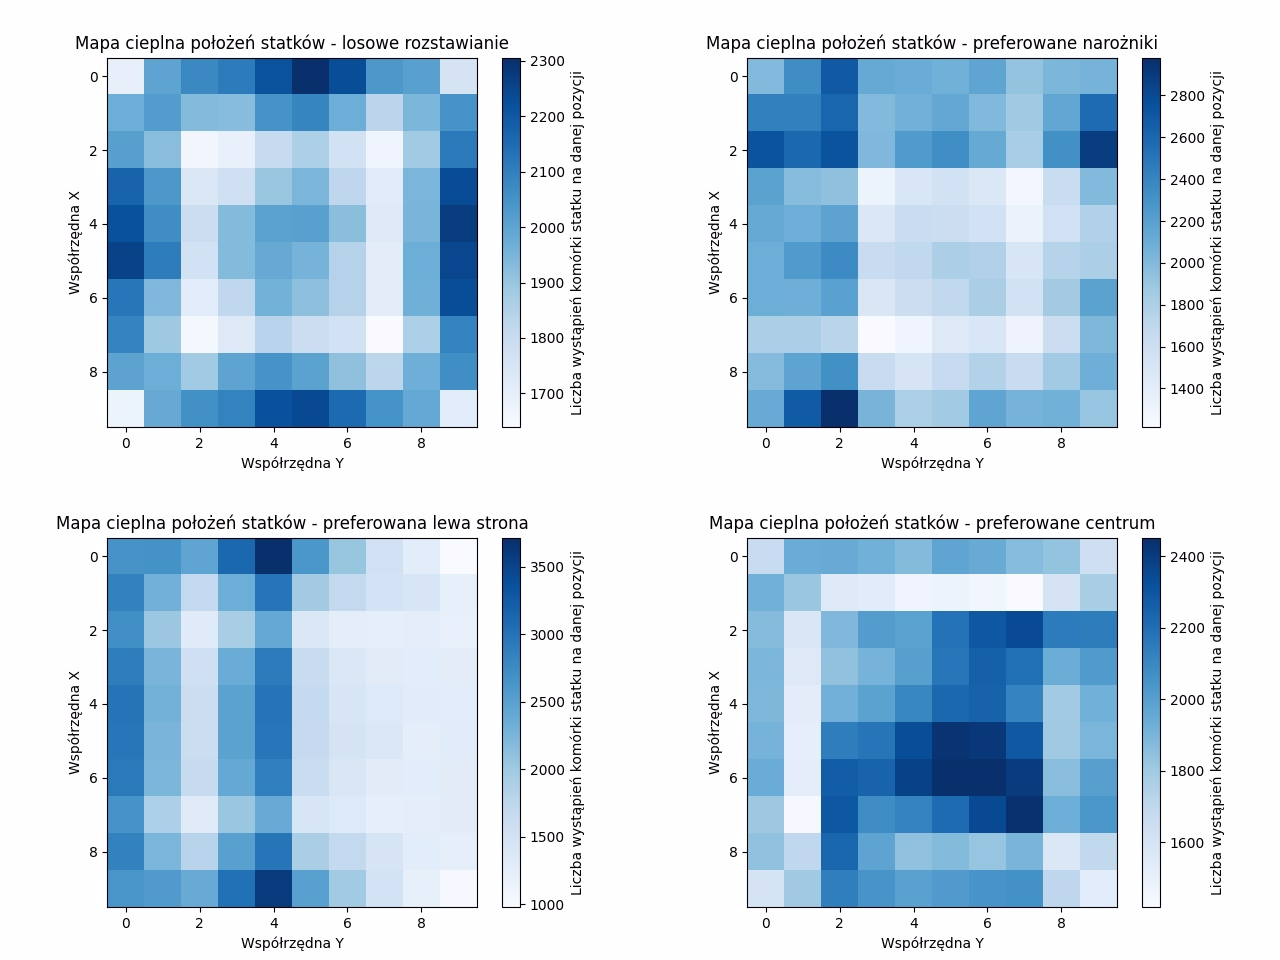
\includegraphics[width=1\linewidth]{img/biases.jpg}
    \caption{Mapy cieplne statków dla różnych tendencji przy rozstawianiu.}
\end{figure}

Na podstawie wyników rozgrywek sporządzono tabele 7.14 i 7.15. Każdy z wierszy opisuje skuteczność danego algorytmu w starciu z identycznym algorytmem, ale wykorzystującym różne tendencje przy rozstawianiu statków. Dla przykładu - komórka odpowiadająca parze "Losowy" - "Narożniki", opisuje skuteczność algorytmu losowego w procentach, przeciwko algorytmowi losowemu, który częściej rozstawia swoje statki w narożnikach planszy. Wszystkie komórki oznaczone są kolorem żółtym, ponieważ nie różnią się o więcej niż 5\% od punktu odniesienia - czyli skuteczności danego algorytmu gdy obie strony losowo rozstawiają statki.

\begin{table}[!h]
    \label{fig:biases-cant-touch}
    \centering 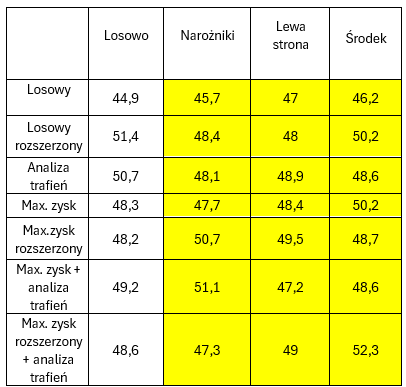
\includegraphics[width=0.7\linewidth]{img/bias_result_cant_touch.png}
    \caption{Skuteczność algorytmów przeciwko sobie dla różnych tendencji rozstawienia statków, gdy statki nie mogą się stykać.}
\end{table}

W tabeli 7.15, podobnie jak w poprzednim przypadku, również nie widać wpływu rozstawienia statków na skuteczność algorytmów.

\begin{table}[!h]
    \label{fig:biases-can-touch}
    \centering 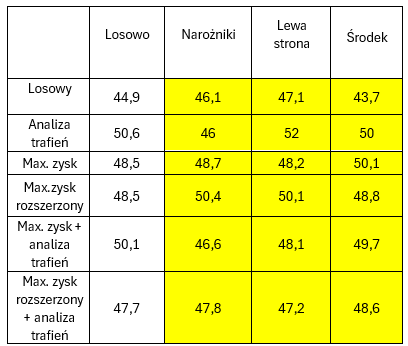
\includegraphics[width=0.7\linewidth]{img/bias_result_can_touch.png}
    \caption{Skuteczność algorytmów przeciwko sobie dla różnych tendencji rozstawienia statków, gdy statki mogą się stykać.}
\end{table}

\subsection{Analiza rozgrywek z ludźmi}

Niestety nie udało się zebrać wystarczająco dużo danych, aby przeprowadzić dokładną analizę skuteczności algorytmów decyzyjnych przeciwko ludziom. Testy algorytm-algorytm opierały się na 1000 rozgrywek pomiędzy parami algorytmów, dla obu wariantów zasad. W przypadku testów z ludźmi, do analizy potrzebnych byłoby 13 000 rozgrywek, ponieważ zaimplementowano 7 algorytmów, w tym jeden który dostępny jest jedynie gdy statki nie mogą się ze sobą stykać. Udało się zebrać dane dotyczące jedynie około 100 rozgrywek, a więc jedynie 1\% potrzebnej liczby. Przeprowadzona na ich podstawie analiza nie jest więc zbyt miarodajna, może być potraktowana raczej jako ciekawostka.

Większość użytkowników preferowała wybór zasad niepozwalających statkom się stykać - dlatego tylko ten przypadek będzie analizowany.

W tabeli 7.14 oraz obrazującym ją wykresie z rysunku 7.12 widać, że ogólna tendencja skuteczności algorytmów jest podobna. Widać jej stopniowy wzrost, oraz spadek średniej liczby tur potrzebnych do pokonania gracza. Anomalią jest znaczny wzrost skuteczności w przypadku algorytmu \emph{Max. zysk}, ale wynika to najprawdopodobniej z małej próby badawczej. Dodatkowym czynnikiem utrudniającym miarodajną analizę wyników starć algorytm-gracz jest fakt, że nie każdy gracz gra na takim samym poziomie. Teoretycznie słabszy algorytm może mieć zawyżoną skuteczność, jeśli grało z nim  więcej 'słabszych' graczy. Dlatego konieczna jest większa ilość rozgrywek, aby wyeliminować wpływ tych czynników na ogół danych.

\begin{table}[!h]
    \label{fig:vs-people}
    \centering 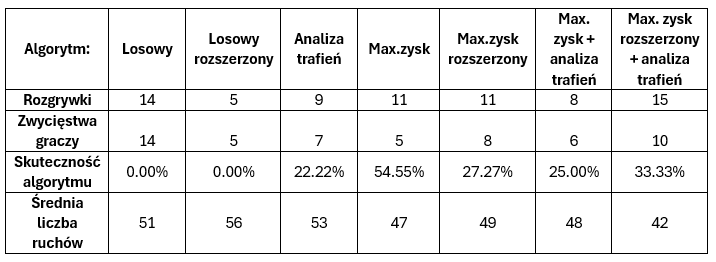
\includegraphics[width=0.9\linewidth]{img/vs_people.PNG}
    \caption{Skuteczność oraz średnia liczba ruchów algorytmów w starciach z graczami.}
\end{table}

\begin{table}[!h]
    \label{fig:vs-people-chart}
    \centering 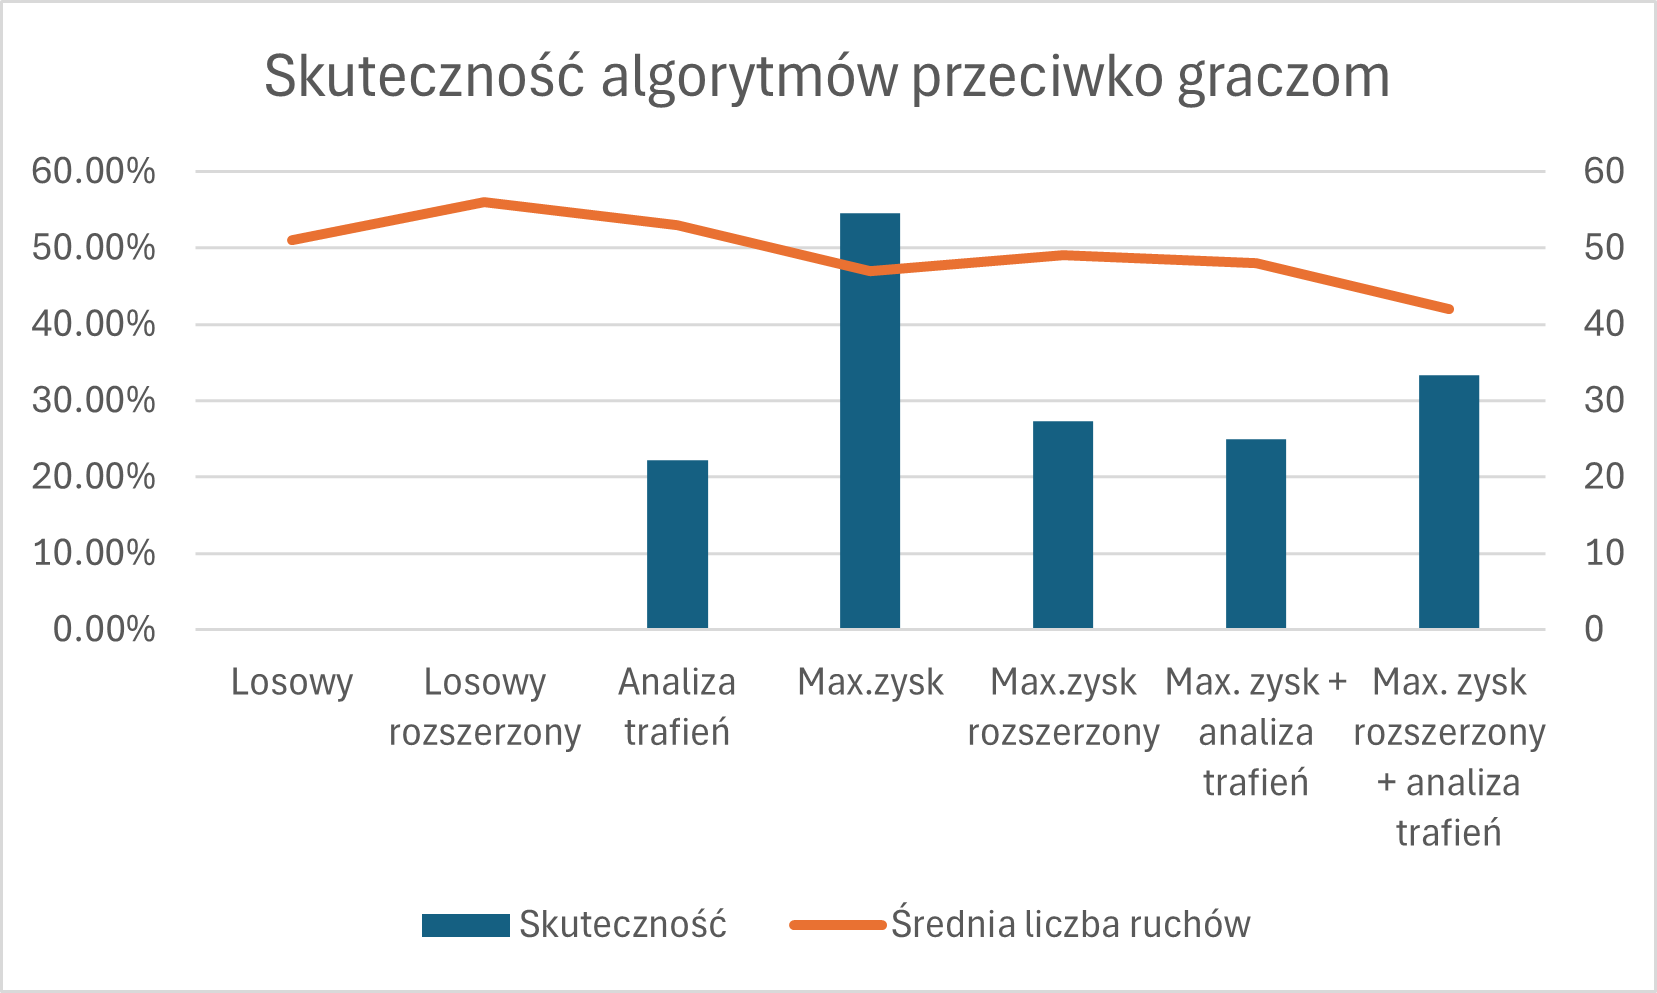
\includegraphics[width=0.9\linewidth]{img/vs_people_chart.png}
    \caption{Wykres przedstawiający skuteczność oraz średnią liczbę ruchów algorytmów w starciach z graczami.}
\end{table}